

	\subsection{Prozesspipelines und Glue Languages} % (fold)
	\label{sub:prozesspipelines_und_glue_languages}
	
	Unix verfolgt das Konzept: \textbf{Alles ist eine Datei}
	\begin{flalign*}
		 \left.\begin{array}{c}
		 	\text{.c}\\
		 	\text{.java}\\
		 	\text{.f77}
		 \end{array}\right\}\text{ Compiler }\rightarrow\text{a.out}
	\end{flalign*}
	Vorteile:
	\begin{itemize}
		\item auch Kompilat braucht keine unterschiedlichen Prozeduren
		\item kein gerätespezifischer Code
	\end{itemize}
	Dateiunabhängig ist damit möglich
	\lstCcode[Lies aus Datei 1 1 Byte und speicher es in c]
	\begin{lstlisting}
read(1,1,&c);
	\end{lstlisting}

	\begin{figure}[hb]
		\caption{Schnittstellen auf System-Ebene zu Abstraktion}
		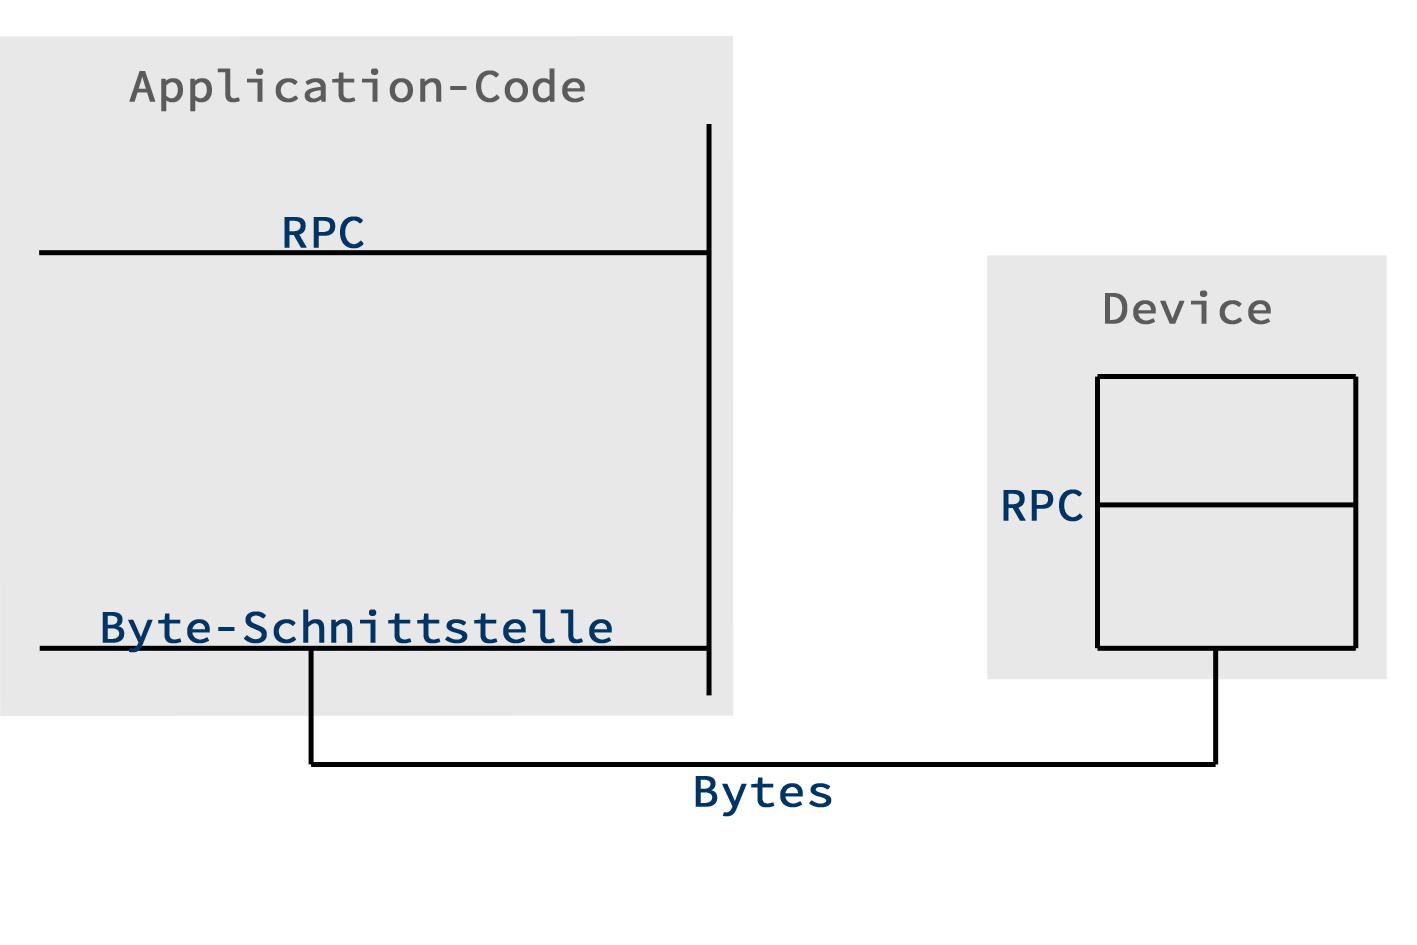
\includegraphics[width=\textwidth]{workfiles/v2_1}
	\end{figure}

	\newpage

	\begin{figure}[h]
		\caption{Hierarchisches Dateisystem}
		\begin{center}
			\tikzstyle{every node}=[anchor=west]
			\begin{tikzpicture}[%
			  grow via three points={one child at (0.5,-0.7) and
			  two children at (0.5,-0.7) and (0.5,-1.4)},
			  edge from parent path={(\tikzparentnode.south) |- (\tikzchildnode.west)}]
			  \node {/}
			    child { node {a}}
			    child { node {b}}
			    child { node {c/}
			      child { node {x}}
			      child { node {y}}
			      child { node {z/}}
			    };
			\end{tikzpicture}
		\end{center}
	\end{figure}

	\begin{figure}[h]
		\caption{Kommunikation zwischen Kernel und Prozess}
		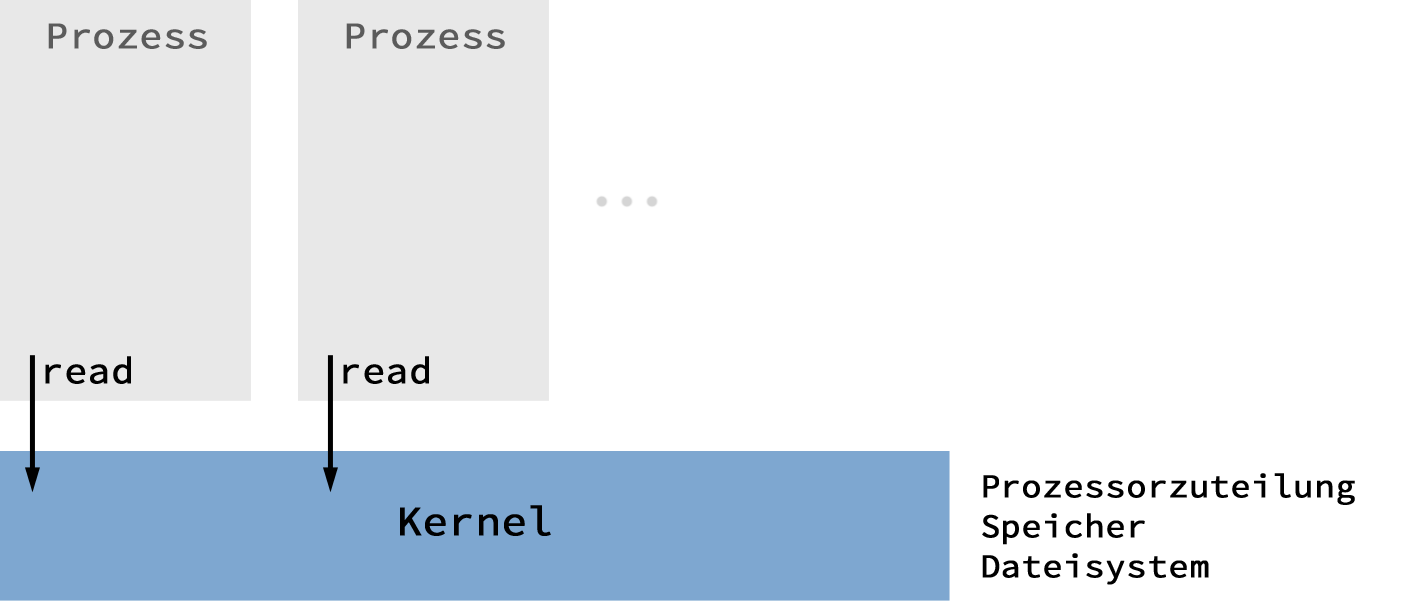
\includegraphics[width=\textwidth]{workfiles/v2_2}
	\end{figure}
	Auch die Shell ist ein Prozess und folgt diesem Kommunikationsschema.\\

	\subsubsection*{Lokaler Dateiaufruf} % (fold)
	\label{ssub:dateiaufrufe}
		
		\lstCcode[Lokaler Dateiufruf]
		\begin{lstlisting}
File *fopen(path)
		\end{lstlisting}

		\begin{figure}[h]
			\caption{Dateiaufruf im Programm}
			
\includegraphics[width=\textwidth]{workfiles/v2_3}
		\end{figure}

		Merkmale des Konzepts
		\begin{itemize}
			\item lokale Aufrufe schneller
			\item andere Prozesse können Datei überschreiben
			\item kein Systemaufruf
			\item werden im Anwendungsprogramm selbst ausgewertet
			\item Versuch auf Buffer zuzugreifen:
				\begin{itemize}
					\item wenn enthalten: gut
					\item wenn nicht: Systemaufruf $\rightarrow$ im Buffer enthalten
				\end{itemize}
			\item wenn der Buffer stückchenweise ausgewertet wird ergeben sich evtl. Veränderungen und er ist nicht mehr aktuell
		\end{itemize}

		\lstCcode[Aufbau einer \texttt{FILE}-Struktur nach \texttt{fopen()}]
		\begin{lstlisting}
f = fopen(path)
f->buf	// Speicher
f->len	// Laenge
f->fd		// File Descriptor
		\end{lstlisting}

	% subsubsection dateiaufrufe (end)

	\subsubsection*{Systemweiter Dateiaufruf} % (fold)
	\label{ssub:systemweiter_dateiaufruf}

		\lstCcode[Systemaufruf]
		\begin{lstlisting}
int open(path)
		\end{lstlisting}

		\begin{itemize}
			\item Systemaufruf, vom Anwendungsprozess wird das Kernel angesprochen
			\item verschiedene Prozesse können nicht gleichzeitig auf das 1. Byte zugreifen
			\item mehrere Prozesse können auf alles weitere häppchenweise zugreifen
			\item es kommt zu einem Kontextwechsel (?)
		\end{itemize}
	
	% subsubsection systemweiter_dateiaufruf (end)

	\subsubsection*{Fork und Exec} % (fold)
	\label{ssub:aufruf_von_fork}
	
		\lstCcode[Welcher Prozess bin ich nach dem \texttt{fork()}?]
		\begin{lstlisting}
if(pid = fork()) {
 // parent
} else {
 // child
}
		\end{lstlisting}

		\lstCcode[Weiterführen mit \texttt{exec()}]
		\begin{lstlisting}
if(pid = fork()) {
 // parent
} else {
 // child
 exec();
}
		\end{lstlisting}

	% subsubsection aufruf_von_fork (end)
	Anmerkungen zu Fork
		\begin{itemize}
			\item um neuen Prozess zu erzeugen
			\begin{itemize}
				\item neuer Eintrag (Memory Map, Prozessor State, File Descriptor)
				\item ALLES wird vom Parent kopiert
			\end{itemize}
				\item wenn parent.fork() $\rightarrow$ id des childs
		\end{itemize}
		
	Anmerkungen zu Exec (path)
		\begin{itemize}
			\item auch ohne vorheriges Fork
			\item path
			\begin{itemize}
				\item[$\rightarrow$] Binärcode des Programms
				\item[$\rightarrow$] neuer Speicherbereich
				\item[$\rightarrow$] dort wird der Code initialisiert
			\end{itemize}
				\item MemoryMap um geschaltet
				\item Zähler/Stackpointer: 0
				\item fängt wieder von Vorne an
		\end{itemize}

	\subsubsection*{Fork und Exec am Beispiel von butfirst.sh} % (fold)
	\label{ssub:fork_am_beispiel_von_butfirst_sh}
	
		\lstShell
		\begin{lstlisting}
#!/bin/sh
read
exec doit
		\end{lstlisting}

		\begin{figure}[th]
			\caption{Ablauf von Fork und Exec}
			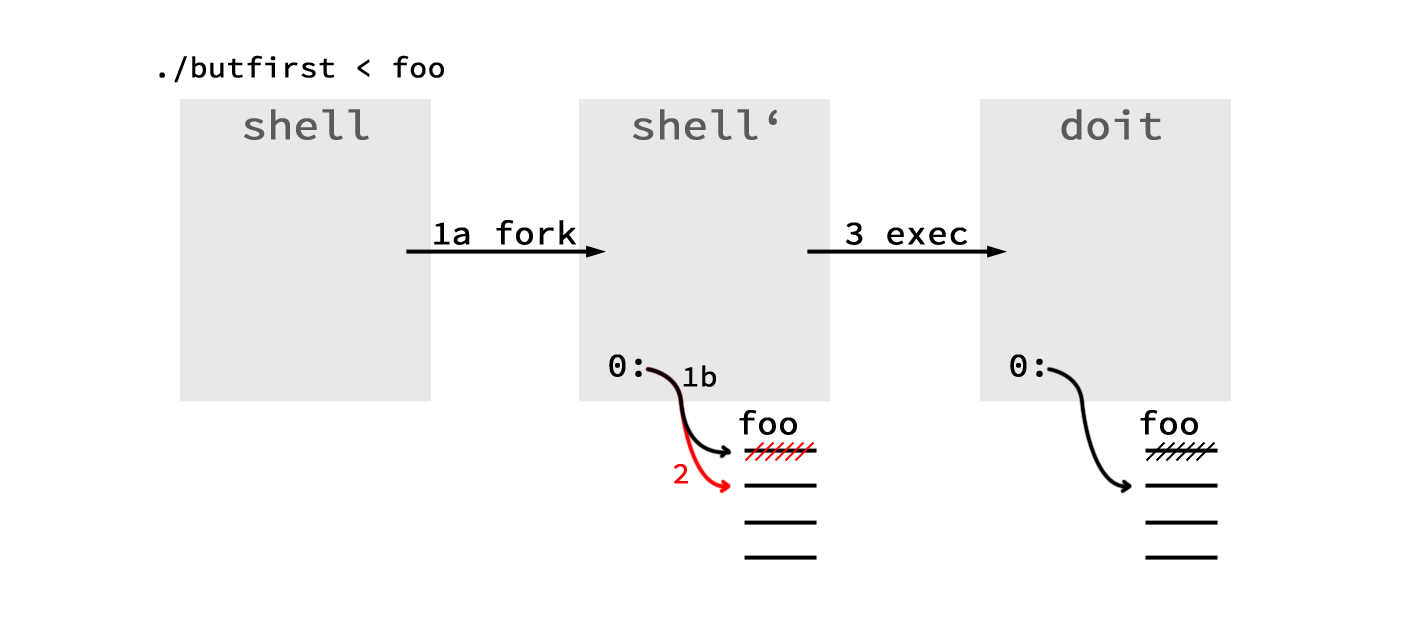
\includegraphics[width=\textwidth]{workfiles/v2_4}
		\end{figure}

	% subsubsection fork_am_beispiel_von_butfirst_sh (end)

	% subsection prozesspipelines_und_glue_languages (end)

	%%%%
	%%%% end V2
	%%%%

	\subsubsection*{Textausgabe in Haskell} % (fold)
	\label{ssub:textausgabe_in_haskell}
	
		\lstHaskell
		\begin{lstlisting}
main = putstrln "Hello World!"
		\end{lstlisting}

		\lstHaskell[Mehrzeilige Ausgabe, Variante 1]
		\begin{lstlisting}
main = putstrln "Hello World!" >> putstrln "Foobar"
		\end{lstlisting}

		\lstHaskell[Mehrzeilige Ausgabe, Variante 2]
		\begin{lstlisting}
main = do {
		putstrln "Hello World!"
		putstrln "Foobar"
	}
		\end{lstlisting}

	% subsubsection textausgabe_in_haskell (end)

	\subsubsection*{Umgebungsvariablen} % (fold)
	\label{ssub:umgebungsvariablen}

		Ausgabe von \texttt{Hello\$USER} ist klar, aber was ist mit \texttt{\$USERHello}?
		\begin{itemize}
			\item gesucht wird nach \texttt{\$USERHello} $\rightarrow$ führt meist zu einem \texttt{not found}
			\item Lösung durch Klammerung: \texttt{\$\{USER\}Hello}
		\end{itemize}

	% subsubsection umgebungsvariablen (end)

	\subsubsection*{Trennzeichen in der Shell} % (fold)
	\label{ssub:trennzeichen_in_der_shell}
	
		Trennzeichen, die in der Varaible \texttt{\$ISF} stehen, werden zur Worttrennung genutzt:
		\lstShell
		\begin{lstlisting}
" \n\t"
		\end{lstlisting}
		Einfaches Ausgeben via \texttt{echo} führt allerdings zu keiner Ausgabe:
		\lstShell
		\begin{lstlisting}
$ echo $IFS
>
		\end{lstlisting}
		Grund: Es sind nur Whitespace-Zeichen, die abgeschnitten werden. Ausgabe als Whitespace möglich (erkennbar an zwei Newlines) über:
		\lstShell
		\begin{lstlisting}
$ echo "$IFS"
>
>
		\end{lstlisting}

	% subsubsection trennzeichen_in_der_shell (end)

	\subsubsection*{Shellübersicht} % (fold)
	\label{ssub:shell_bersicht}
	
		\begin{tabular}{lll}
			bash	&	Bourne Again Shell 	&	in Vorlesung genutzt\\
			sh		&	Bourne Shell 		&	ursrüngliche Shell\\
			csh		&	c Shell 			&	\\
			ksh		&	Korn Shell 			&	
		\end{tabular}

	% subsubsection shell_bersicht (end)

	\subsubsection*{True und False in der Shell} % (fold)
	\label{ssub:true_und_false_in_der_shell}
	
		In der Shell sind auch \texttt{true} und \texttt{false} ausführbare Programme.
		\lstCcode[\texttt{true} als C-Programm]
		\begin{lstlisting}
int main() { return 0; }
		\end{lstlisting}

	% subsubsection true_und_false_in_der_shell (end)

	\subsubsection*{Vorsicht vor deprecated Befehlen} % (fold)
	\label{ssub:vorsicht_vor_deprecated_befehlen}
	
		Veraltete Befehle können Sicherheitsrisiken sein. Beispiel \texttt{gets()}:

		\lstCcode[testpwd.c]
		\begin{lstlisting}
getInp() {
	char buff[1000];
	gets(buff);
}
		\end{lstlisting}
		\begin{figure}[hbtp]
			\caption{Illustrations des gets-Problems}
			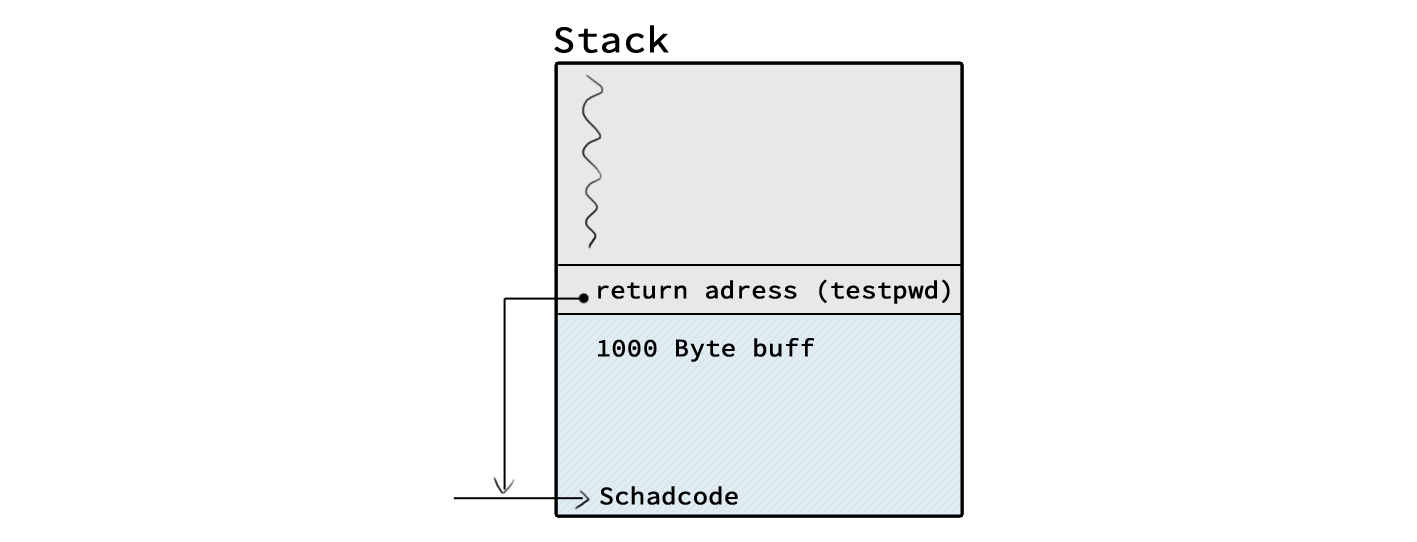
\includegraphics[width=\textwidth]{workfiles/v3_1}
		\end{figure}

	% subsubsection vorsicht_vor_deprecated_befehlen (end)

	\subsubsection*{Dateiumleitungen} % (fold)
	\label{ssub:dateiumleitungen}
	
		\begin{tabular}{ll}
			\texttt{> file}		&	in \texttt{file} leiten	\\
			\texttt{>> file}	&	an \texttt{file} anfügen	\\
			\texttt{< file}		&	aus \texttt{file} lesen	\\
			\texttt{1 > file}	&	File Descriptor 1 leitet in \texttt{file}	\\
			\texttt{2 >\& 1}	&	FD2 leitet in selbes Ziel wie FD 1	\\
			\texttt{FD0}		&	Standardinput	\\
			\texttt{FD1}		&	Standardoutput	\\
			\texttt{FD2}		&	Standarfehlerausgabe	\\
		\end{tabular}

		\begin{flalign*}
			&\text{\texttt{printf("Hello$\backslash$n");}}	\\
			&\qquad\downarrow	\\
			&\text{\texttt{FILE *stdout}}	\\
			&\qquad\downarrow	\\
			&\text{\texttt{write(stdout->fd, stdout->buf, stdout->len);}}
		\end{flalign*}

	% subsubsection dateiumleitungen (end)

	%%%%
	%%%% end V3
	%%%%